% !TEX root = ../vr_st.tex

%Let $X$ be an $\R$-space where $X_r$ is empty for $r<0$ and contractible for $r\geq R$ for some real number $R$.
%The Vietoris--Rips complex of a metric space is our primary example.
%In this subsection, we will consider this $\R$-space and omit it from the notation when convenient.

\subsection{Kuratowski embedding and critical radii}\label{sub:filling radii}

\subsubsection{}

Any compact metric space $\cX$ can be isometrically embedded into the space $\rL^\infty(\cX)$ of all bounded real-valued functions on $\cX$ via the map $x \in \cX \mapsto d_\cX(x,\cdot)$, the so-called \defn{Kuratowski embedding}.
We are interested in the \(\R\)-space obtained by considering radius \(r\) neighborhoods of the image of \(\cX\), which we denote \(\rU_r(\cX)\).

Throughout the text, Riemannian manifolds are thought of as metric spaces with the geodesic distance.

\subsubsection{}\label{ss:first_critical_value}

Let \(\cM\) be a closed Riemannian manifold.
By \cite[Thm.~3.5]{hausmann1995vietoris} and \cite[Thm.~4.1]{lim2024vietoris}, we know that there exists \(r_\cM > 0\) such that for all \(r \in (0,r_\cM)\) the inclusion \(\cM \to \rU_r(\cM)\) is a homotopy equivalence.
We define the \defn{homotopical radius} of \(\cM\), denoted by \(\Rad_{htpy}(\cM)\), as the supremum among all such real numbers.

\ling{I will use commands for all critical values. 
`fillrad' for filling radius; `crit' for homotopy radius; `firstdeath' for both homological radius and image of theta. Please change the corresponding commands if you would like to change the notations later on.} 

%Clearly, if \(\cM\) is connected we have
%\[
%\crit(\cM) \leq \Rad(\cM).
%\]

\subsubsection{}

Following \cite{gromov1983filling}, the \defn{filling radius} of an \(n\)-dimensional closed orientable Riemannian manifold $\cM$, denoted \(\fillrad(\cM)\), is defined as the infimal $\epsilon > 0$ such that the fundamental class in $\rH_n(M; \Z)$ is mapped to zero by the inclusion $\cM \hookrightarrow \rU_\epsilon(\cM)$, where \(\rU_\epsilon(\cM)\) is the \(\epsilon\)-neighborhood of \(\cM\) in \(\rL^\infty(\cX)\).
For connected non-orientable manifolds, the filling radius is defined similarly using mod~2 coefficients.
Notice that, in this case,
\[
\fillrad(\cM) = \min\set[\big]{r \mid (0, r) \in \barc \rH_n(\rU(\cM); \Ftwo)}.
\]

\subsubsection{}

Let us fix a field \(\bK\) and an integer \(m \in \N\), the \defn{\(m\)-homological radius} of a totally bounded metric space \(\cX\) is defined by

%\(\Rad_m(\cM; \bF)\) is defined as follows.
%If \(\rH_\degp(\cM) = 0\), set \(\Rad_m(\cM) = 0\), and if not, let \(\Rad_m(\cM)\) be the smallest positive radius $r$ for which a non-zero homology class in \(\rH_\degp(\cM)\) becomes \(0\) in \(U_r(\cM)\).
%Since \(\VR(\cM)\) is \(q\)-tame,
\[
\firstdeath{m}{\cX; \bK} = \min\set[\big]{r \mid (0, r) \in \barc \rH_m(\rU(\cM); \bK)}.
\]
We will omit \(\bK\) from the notation when clear from the context.

%Clearly, if \(\rH_m(\cM) \neq 0\),
%\[
%\crit(\cM) \leq 2 \cdot \Rad_m(\cM).
%\]
Similarly, for a linear cohomology operation \(\theta\), we define the \defn{\(\img_\theta\)-radius} of \(\cX\) by
\[
\firstdeath{\theta}{\cX} = \min\set[\big]{r \mid (0, r) \in \barc \img_\theta(\rU(\cX))}.
\]
The \(\ker_\theta\)-radius could be defined similarly, but we do not use it in this work.

\anibal{Please study this label: \{subsub:beta v.s. fillrad\}. I.e., where is it used and what to cite instead.
\ling{The label is needed to refer to what is commented out below:}}

%and observe that
%\[
%\crit(\cM) \leq 2 \cdot \Rad_\theta(\cM))
%\]
%if \(\img_\theta(\cM) \neq 0\).

%\subsubsection{}
%
%If \(\rH_\degp(\cM) = 0\), set \(\Rad_m(\cM) = 0\), and if not, let \(\Rad_m(\cM)\) be the smallest positive radius $r$ for which a non-zero homology class in \(\rH_\degp(\cM)\) becomes \(0\) in \(U_r(\cM)\).
%Since \(\VR(\cM)\) is \(q\)-tame,
%\[
%\Rad_m(\cM) = \min\set[\big]{r \mid (0, 2r) \in \barc \rH^{\VR}_m(\cM)}.
%\]
%Clearly, if \(\rH_m(\cM) \neq 0\),
%\[
%\crit(\cM) \leq 2 \cdot \Rad_m(\cM).
%\]
%Similarly, for a linear cohomology operation \(\theta\), we define
%\[
%\Rad_\theta(\cM) = \min\set[\big]{r \mid (0, 2r) \in \barc \img_\theta^{\!\VR}(\cM)}
%\]
%and observe that
%\[
%\crit(\cM) \leq 2 \cdot \Rad_\theta(\cM))
%\]
%if \(\img_\theta(\cM) \neq 0\).

%\ling{Just a warning that we restrict ourselves to only talking about the critical values of manifolds. This seems fine. The only non-manifold spaces we are studying are wedge sums of sphes, whosree barcodes are obtained by taking unions of barcodes of spheres.}

%\subsubsection{}

%Let us assume \(\cM\) connected.
%Since, as stated in \cref{ss:kuratowski_vr}, \(\VR_{2r}(\cM)\) is homotopy equivalent to \(U_r(\cM) \subset \rL^\infty(\cM)\), an upper bound for \(\crit(\cM)\) is \(2\cdot\Rad(\cM)\).
%
%We generalize this from the top homology to every other degree \(\degp\) and to non-connected manifolds so that
%\[
%\Rad_\degp(\cM) = \Rad(\cM)
%\]
%if \(\cM\) is connected and \(\degp\)-dimensional.

%\ling{I think the notation $\Rad$ is too suggestive. It is a quantity we `create' to describe the barcode estimates. It might have deeper meanings, but we are not present those.}

\subsection{Vietoris--Rips filtrations}

\subsubsection{}\label{ss:kuratowski_vr}

As proven in \cite[Thm.~4.1]{lim2024vietoris}, there is deep relationship between the \(r\)-neighborhood filtration of $\cX$ in $\rL^\infty(\cX)$ and the Vietoris--Rips complex of \(\cX\) at distance \(2r\), stated in the following.

\medskip\lemma The spaces $\VR_{2r}(\cX)$ and $\rU_r(\cX)$ are naturally homotopy equivalent for every \(r > 0\).

\subsubsection{}

The previous natural homotopy equivalence gives rise to the following result proven in \cite[Prop.~9.28]{lim2024vietoris}.

\medskip\lemma
If $\cM$ is a closed connected $n$-dimensional Riemannian manifold, then \(\Hbarc{n}{\cM}\) contains the bar \((0,2\fillrad(\cM))\) for arbitrary field coefficients if $M$ is orientable, and for mod $2$ coefficients $M$ if not.\anibal{Fix interval please }
Moreover, this is the unique bar in \(\Hbarc{n}{\cM}\) starting at $0$.


\subsection{General estimates}\label{ss:barcode_general}

Let \(\cM\) be a closed Riemannian manifold with diameter \(R\).
Consider \(\ell, \degp \in \N\) and \(\theta \in \cO(\ell,\degp)\).
We will simplify notation writing \(\alpha = \crit(\cM)\), \(\beta_m = \firstdeath{\degp}{\cM}\), and \(\gamma_\theta = \firstdeath{\theta}{\cM}\).

Because $\VR_r(\cM)$ is empty for \(r \leq 0\) and the homotopy type of $\VR_r(\cM)$ remains the homotopy type of $\cM$ for $r \in (0, \alpha)$, bars in \(\barc \rH_\degp^{\VR}(\cM)\) and $\barc\img_\theta^{\VR}(\cM)$ either start at $0$ or start after $\alpha$.

More precisely,
%we estimate the reduced homology barcode of $\cM$ by considering two cases.
if \(k = \dim \opH_\degp(\cM) > 0\) then $\barc\rH_\degp^{\VR}(\cM)$ contains $(0, \beta_m)$ and \((k - 1)\) additional bars of the form \((0, b)\) with \(\beta_m \leq b \leq R\).
Additionally, all other bars are dominated by \((\alpha, R)\).
Recall that a bar $(a, b)$ is said to be dominated by another $(c,d)$ if $c \leq a < b \leq d$.
If \(\dim \opH_\degp(\cM) = 0\) then all bars in \(\barc\rH_\degp^{\VR}(\cM)\) are dominated by \((\alpha, R)\).
See the first row of \cref{fig:barcodes_general} for a pictorial representation of these estimates.

A similar analysis applies to $\barc\img_\theta^{\VR}(\cM)$.
See the second row of \cref{fig:barcodes_general} for these estimates.

\begin{figure}
	\centering
	\begin{tikzpicture}[scale=0.52]
	\begin{axis} [
		title = {\LARGE $\barc\opH_m^{\VR}(\cM)$, if $\opH_m(\cM) \neq 0$},
		ticklabel style = {font=\Large},
		axis y line=middle,
		axis x line=middle,
		ytick={0.7,0.95},
		yticklabels={$2\firstdeath{m}{\cM}$,$\diam(\cM)$},
		xtick={0.55,0.95},
		xticklabels={$2\crit(\cM)$, $\diam(\cM)$},
		xmin=-0.015, xmax=1.1,
		ymin=0, ymax=1.1,]
		\addplot [mark=none] coordinates {(0,0) (1,1)};
		\addplot [thick,color=black!20!white,fill=black!30!white,
		fill opacity=0.4]coordinates {
			(0.55,0.95)
			(0.55,0.55)
			(0.95,0.95)
			(0.55,0.95)};
		\addplot [black!40!white,mark=none,dashed, thin] coordinates {(0,0.7) (0.7,0.7)};
		\addplot [black!40!white,mark=none,dashed, thin] coordinates {(0,0.55) (0.55,0.55)};
		\addplot [black!40!white,mark=none,dashed, thin] coordinates {(0.55,0) (0.55,0.55)};
		\addplot[line width=1.5mm, color=black!30!white] coordinates{(0, 0.7) (0, 0.95)};
		\addplot[barccolor,mark=*] (0, 0.7) circle (2pt) node[above right,barccolor]{};
	\end{axis}
\end{tikzpicture}
\begin{tikzpicture}[scale=0.52]
	\begin{axis} [
		title = {\LARGE $\barc\opH_m^{\VR}(\cM)$, if $\opH_m(\cM) = 0$},
		ticklabel style = {font=\Large},
		axis y line=middle,
		axis x line=middle,
		ytick={0.95},
		yticklabels={$\diam(\cM)$},
		xtick={0.55,0.95},
		xticklabels={$2\crit(\cM)$, $\diam(\cM)$},
		xmin=-0.015, xmax=1.1,
		ymin=0, ymax=1.1,]
		\addplot [mark=none] coordinates {(0,0) (1,1)};
		\addplot [thick,color=black!20!white,fill=black!30!white,
		fill opacity=0.4]coordinates {
			(0.55,0.95)
			(0.55,0.55)
			(0.95,0.95)
			(0.55,0.95)};
		\addplot [black!40!white,mark=none,dashed, thin] coordinates {(0,0.55) (0.55,0.55)};
		\addplot [black!40!white,mark=none,dashed, thin] coordinates {(0.55,0) (0.55,0.55)};
	\end{axis}
\end{tikzpicture}

\begin{tikzpicture}[scale=0.52]
	\begin{axis} [
		title={\LARGE $\thetabarc{\cM}$, if $\img\theta_{\cM}\neq 0$},
		ticklabel style = {font=\Large},
		axis y line=middle,
		axis x line=middle,
		ytick={0.7,0.95},
		yticklabels={$2\firstdeath{\theta}{\cM}$,$\diam(\cM)$},
		xtick={0.55,0.95},
		xticklabels={$2\crit(\cM)$, $\diam(\cM)$},
		xmin=-0.015, xmax=1.1,
		ymin=0, ymax=1.1,]
		\addplot [mark=none] coordinates {(0,0) (1,1)};
		\addplot [thick,color=black!20!white,fill=black!30!white,
		fill opacity=0.4]coordinates {
			(0.55,0.95)
			(0.55,0.55)
			(0.95,0.95)
			(0.55,0.95)};
		\addplot [black!40!white,mark=none,dashed, thin] coordinates {(0,0.7) (0.7,0.7)};
		\addplot [black!40!white,mark=none,dashed, thin] coordinates {(0,0.55) (0.55,0.55)};
		\addplot [black!40!white,mark=none,dashed, thin] coordinates {(0.55,0) (0.55,0.55)};
		\addplot[line width=1.5mm, color=black!30!white] coordinates{(0, 0.7) (0, 0.95)};
		\addplot[barccolor,mark=*] (0, 0.7) circle (2pt) node[above right,barccolor]{};
	\end{axis}
\end{tikzpicture}
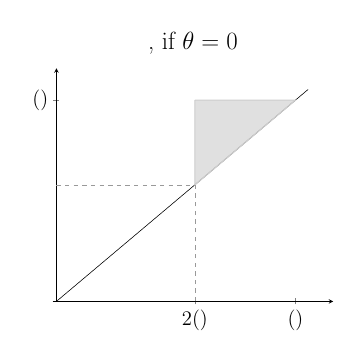
\begin{tikzpicture}[scale=0.52]
	\begin{axis} [
		title={\LARGE $\thetabarc{\cM}$, if $\img\theta_{\cM}= 0$},
		ticklabel style = {font=\Large},
		axis y line=middle,
		axis x line=middle,
		ytick={0.95},
		yticklabels={$\diam(\cM)$},
		xtick={0.55,0.95},
		xticklabels={$2\crit(\cM)$, $\diam(\cM)$},
		xmin=-0.015, xmax=1.1,
		ymin=0, ymax=1.1,]
		\addplot [mark=none] coordinates {(0,0) (1,1)};
		\addplot [thick,color=black!20!white,fill=black!30!white,
		fill opacity=0.4]coordinates {
			(0.55,0.95)
			(0.55,0.55)
			(0.95,0.95)
			(0.55,0.95)};
		\addplot [black!40!white,mark=none,dashed, thin] coordinates {(0,0.55) (0.55,0.55)};
		\addplot [black!40!white,mark=none,dashed, thin] coordinates {(0.55,0) (0.55,0.55)};
	\end{axis}
\end{tikzpicture}
	\caption{In each figure, the gray region represents where additional bars could potentially exist within the corresponding barcode.}
	\label{fig:barcodes_general}
\end{figure}